%%%%%%%%%%%%%%%%%%%%%%%%%%%%%%%%%%%%%%%%%
% Thin Sectioned Essay
% LaTeX Template
% Version 1.0 (3/8/13)
%
% This template has been downloaded from:
% http://www.LaTeXTemplates.com
%
% Original Author:
% Nicolas Diaz (nsdiaz@uc.cl) with extensive modifications by:
% Vel (vel@latextemplates.com)
%
% License:
% CC BY-NC-SA 3.0 (http://creativecommons.org/licenses/by-nc-sa/3.0/)
%
%%%%%%%%%%%%%%%%%%%%%%%%%%%%%%%%%%%%%%%%%

%----------------------------------------------------------------------------------------
%	PACKAGES AND OTHER DOCUMENT CONFIGURATIONS
%----------------------------------------------------------------------------------------

\documentclass[a4paper, 11pt]{article} % Font size (can be 10pt, 11pt or 12pt) and paper size (remove a4paper for US letter paper)

\usepackage[protrusion=true,expansion=true]{microtype} % Better typography
\usepackage{graphicx} % Required for including pictures
\usepackage{wrapfig} % Allows in-line images
\usepackage{subfigure}
\usepackage{mathpazo} % Use the Palatino font
\usepackage[T1]{fontenc} % Required for accented characters
\linespread{1.05} % Change line spacing here, Palatino benefits from a slight increase by default

\makeatletter
\renewcommand\@biblabel[1]{\textbf{#1.}} % Change the square brackets for each bibliography item from '[1]' to '1.'
\renewcommand{\@listI}{\itemsep=0pt} % Reduce the space between items in the itemize and enumerate environments and the bibliography

\renewcommand{\maketitle}{ % Customize the title - do not edit title and author name here, see the TITLE block below
\begin{flushright} % Right align
{\LARGE\@title} % Increase the font size of the title

\vspace{50pt} % Some vertical space between the title and author name

{\large\@author} % Author name
\\\@date % Date

\vspace{40pt} % Some vertical space between the author block and abstract
\end{flushright}
}

%----------------------------------------------------------------------------------------
%	TITLE
%----------------------------------------------------------------------------------------

\title{\textbf{Self-Organizing Map}\\ % Title
HW4 of Neural Network} % Subtitle

\author{\textsc{Yang Guang} % Author
\\{\textit{1140339072}}} % Institution

\date{\today} % Date




%----------------------------------------------------------------------------------------

\begin{document}

\maketitle % Print the title section

%----------------------------------------------------------------------------------------
%	ABSTRACT AND KEYWORDS
%----------------------------------------------------------------------------------------

%\renewcommand{\abstractname}{Summary} % Uncomment to change the name of the abstract to something else




%----------------------------------------------------------------------------------------
%	ESSAY BODY
%----------------------------------------------------------------------------------------

\section*{Introduction of SOM}

Self-Organizing Map is trained using unsupervised learning to produce a low-dimensional (typically two-dimensional), discretized representation of the input space of the training samples, called a map. This makes SOMs useful for visualizing low-dimensional views of high-dimensional data, akin to multidimensional scaling. In this work we will focus on an Matlab implementation of SOM based on the given data source in the form of 5 X 5 neurons.
The whole processing of SOM can be listed as follows:
\begin{enumerate}
	\item Initialize each node's weights 
	\item Choose a random vector from training data and present it to the SOM.
	\item Every node is examined to find the Best Matching Unit (BMU). In our experiment, we just choose the node with minimal distance as the Best Matching Unit.
	\item The radius of the neighborhood around the BMU is calculated. The size of the neighborhood decreases with each iteration.
	\item Each node in the BMU's neighborhood has its weights adjusted to become more like the BMU. Nodes closest to the BMU are altered more than the nodes furthest away in the neighborhood. The updating rule can also be formulized as follows:
		$m_k = m_k + \alpha h(\parallel m_j - m_k \parallel)(x_j - m_k)$
	where $m_j$ is the BMU, $m_k$ is the node to be updated, $\alpha$ is the learning rate, $x_j$ is the data sample presented to SOM, $h$ is the neighbor function which gives the similarity of $m_j$ and $m_k$.
	\item Repeat from step 2 for enough iterations for convergence. 
\end{enumerate}

%------------------------------------------------

\section*{Implementation and Result of SOM}
We using a 5 X 5 neurons with 2000 epoch as a maximum iteration.
The folling figures are token from epoch 1, 10, 100, 1000 and 2000. We can clearly view a procedure of convergence.

\begin{figure}[h]
	\centering 
	\subfigure[1 epoch]{ 
		\label{fig:subfig:a} 
		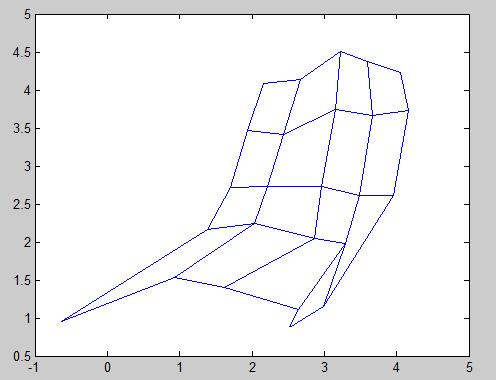
\includegraphics[width=0.3\linewidth]{1.png}} 
	\subfigure[10 epoch]{
		\label{fig:subfig:b} 
		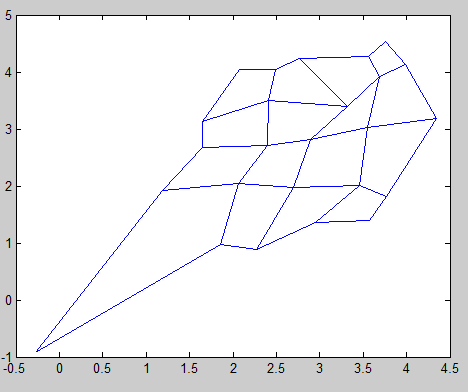
\includegraphics[width=0.3\linewidth]{10.png}}
	\subfigure[100 epoch]{
		\label{fig:subfig:d} 
		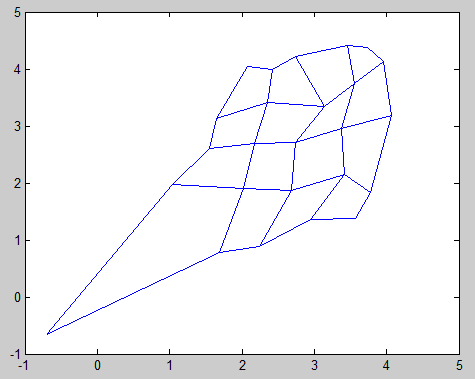
\includegraphics[width=0.3\linewidth]{100.png}}
	\subfigure[1000 epoch]{ 
		\label{fig:subfig:e} 
		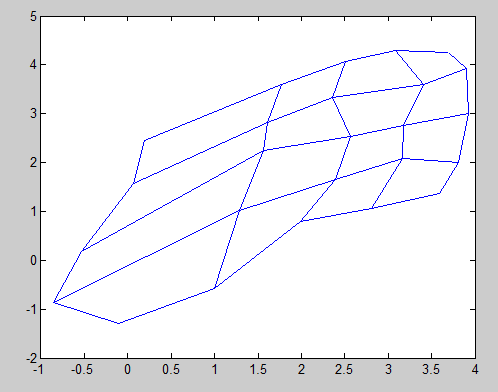
\includegraphics[width=0.3\linewidth]{1000.png}} 
	\subfigure[2000 epoch]{
		\label{fig:subfig:f} 
		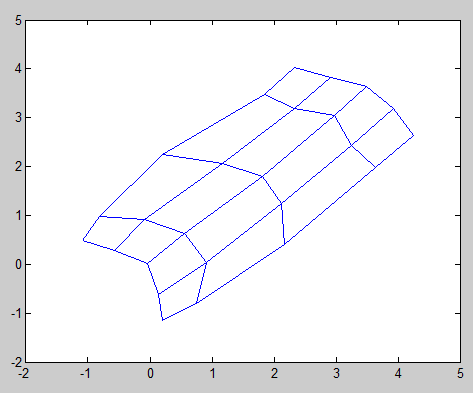
\includegraphics[width=0.3\linewidth]{2000.png}}
	\caption{The coordinate of the centers}
	\label{fig:subfig}
\end{figure}

%----------------------------------------------------------------------------------------

\end{document}